    % !TEX program = lualatex
\PassOptionsToPackage{naturalnames}{hyperref}
\RequirePackage{luatex85}
\documentclass{article}
\usepackage{geometry}
%\usepackage{fullpage}
\usepackage{parskip}
\usepackage{physics}
\usepackage{amsmath}
\usepackage{amssymb}
\usepackage{xcolor}
\usepackage[colorlinks,linkcolor=blue,citecolor=green]{hyperref}
\usepackage{array}
\usepackage{longtable}
\usepackage{multirow}
\usepackage{comment}
\usepackage{graphicx}
\usepackage{cite}
\usepackage{amsfonts}
\usepackage{bm}
\usepackage{slashed}
\usepackage{dsfont}
\usepackage{mathtools}
\usepackage[compat=1.1.0]{tikz-feynman}
\usepackage{simplewick}
%\usepackage{fourier}
%\usepackage{slashbox}
%\usepackage{intent}
\usepackage{mathrsfs}
\usepackage{xparse}
\usepackage{enumerate}
%\usepackage{axodraw4j}
\usepackage[toc,page]{appendix}
\usepackage{multicol}
\usepackage{authblk}
\usepackage[T1]{fontenc}
%\usepackage[utf8]{inputenc}

%\usepackage{luatexja-fontspec}

\geometry{left=1.3cm,right=1.3cm,top=1.5cm,bottom=2cm}

\newcommand{\gm}{\gamma^{\mu}}
\newcommand{\gn}{\gamma^{\nu}}
\newcommand{\gs}{\gamma^{\sigma}}
\newcommand{\gr}{\gamma^{\rho}}
\newcommand{\gnr}{g^{\nu\rho}}
\newcommand{\gmr}{g^{\mu\rho}}
\newcommand{\gms}{g^{\mu\sigma}}
\newcommand{\gns}{g^{\nu\sigma}}
\newcommand{\vbp}{\vb{p}}
\newcommand{\vbk}{\vb{k}}
\newcommand{\g}{\gamma}
\renewcommand{\a}{\alpha}
\renewcommand{\b}{\beta}
\renewcommand{\t}{\theta}
\newcommand{\la}{\lambda}
\newcommand{\p}{\phi}
\newcommand{\vp}{\varphi}
\newcommand{\s}{\sigma}
\newcommand{\G}{\Gamma}
\newcommand{\pars}{\slashed\partial}
\newcommand{\ps}{\slashed p}
\newcommand{\ks}{\slashed k}
\newcommand{\lag}{\mathcal{L}}
\newcommand{\da}{^{\dagger}}
\newcommand{\sm}{^{\mu}}
\newcommand{\sn}{^{\nu}}
\newcommand{\smn}{^{\mu\nu}}
\newcommand{\Dm}{D^{\mu}}
\newcommand{\dm}{\partial^{\mu}}
\newcommand{\Asquare}{A^{\mu}A_{\mu}}
\newcommand{\partialsquare}[2]{\partial^{\mu}{#1}\partial_{\mu}{#2}}

%\setmainjfont[BoldFont=FandolSong-Bold]{FandolSong-Regular}
%\setsansjfont{FandolSong-Bold}
%\setlength{\parindent}{2em}
%\linespread{1.2}
%\renewcommand\Authsep{, }

\title{NRQED}
\author{Yingsheng Huang and Rui Yu}

\begin{document}
\maketitle
\section{Hydrogen Wavefunction Divergence Near Origin in Dirac Equation and Schr\"odinger Equation}
\subsection{The Dirac part}
The Dirac Hydrogen Equation is
\begin{align}
	(\bm{\a}\cdot \vbp+\b m-\frac{Z\a}{r} )\Psi=E\Psi
\end{align}

For the bound state, the wavefunction is
\begin{align}
	\Psi^+_{1,\frac{1}{2},\frac{1}{2}}  & =\bmqty{\frac{ic\sqrt{m+E}\rho^{\gamma}e^{-\frac{\rho}{2}}}{r}\sqrt{\frac{1}{4\pi}}\bmqty{1 \\0}\\-\frac{c\sqrt{m-E}\rho^{\gamma}e^{-\frac{\rho}{2}}}{r}\sqrt{\frac{1}{4\pi}}\bmqty{\cos\theta\\\sin\theta e^{i\phi}}}\\
	\Psi^+_{1,\frac{1}{2},-\frac{1}{2}} & =\bmqty{\frac{ic\sqrt{m+E}\rho^{\gamma}e^{-\frac{\rho}{2}}}{r}\sqrt{\frac{1}{4\pi}}\bmqty{0 \\1}\\-\frac{c\sqrt{m-E}\rho^{\gamma}e^{-\frac{\rho}{2}}}{r}\sqrt{\frac{1}{4\pi}}\bmqty{\sin\theta e^{i\phi}\\\cos\theta}}
\end{align}
where
\begin{align}
	E=m\gamma,\;\rho=2\lambda r,\;\lambda=mZ\a,\;
	\gamma=\sqrt{1-Z^2\a^2},\;c=\sqrt{\frac{Z\a}{\Gamma(2\gamma+1)}}
\end{align}
c is the normalization factor for $\int d^3r|\Psi|^2=1$. 

Only keeping the upper component $\psi_u$, we need to normalize it again so that $\int d^3r\psi_u^2=1$. We get an extra normalization factor
$$1-\frac{\lambda^2}{8m^2}+\frac{2\gamma\lambda}{4m^2r}-\frac{\gamma^2-\gamma}{8m^2r^2}$$

For convenience, define
\begin{align}
	\Psi '=\frac{\Psi}{2(mZ\alpha)^\frac{3}{2}}
\end{align}

Now $\Psi '$ is dimensionless and expand it in $\alpha$, we get the origin divergence comes from a term
\begin{align}
	-(Z\alpha)^2\log(m r)
\end{align}
the $m$ in $\log$ could be interpreted as a subtraction point $\mu$.

\subsection{The Schr\"odinger part}

The Hamiltonian is

\begin{align}
	H & =H_0+H_{int}                                                                                                                            \\
	H & _0=-\frac{\nabla^2}{2m}-\frac{Z\alpha}{r},\ \ \ H_{int}=\frac{\nabla^4}{8m^3}-\frac{1}{8m^2}\nabla^2\frac{Z\a}{r}+\frac{1}{4m^2}\frac{Z\a}{r^3}\bm{\s}\cdot\vb{L}
\end{align}

The first term of $H_{int}$ is the relativistic kinematic $v^2$ correction, the second one is the Darwin term.\\
The $H_0$ gives the radial wave functions as follows
\begin{align}
	R_{n0} & =\frac{2(mZ\alpha)^\frac{3}{2}}{n^\frac{3}{2}}e^{-\frac{mZ\alpha}{n}r}F(1-n,2,\frac{2mZ\alpha r}{n}),\ \ \ E_n=-\frac{Z^2\alpha^2m}{2n^2}                                \\
	R_{k0} & =\sqrt{\frac{2}{\pi}}(mZ\alpha)^\frac{3}{2}ke^\frac{\pi}{2k}|\Gamma(1-\frac{i}{k})|e^{-imz\alpha kr}F(1+\frac{i}{k},2,2imZ\alpha kr),\ \ \ E_k=\frac{mZ^2\alpha^2k^2}{2}
\end{align}

Within perturbation theory,$E_1^{(1)}=<\phi|H_{int}|\phi>$, in quantum mechanics, the NLO energy correction is
\begin{align}
	E_1^{(1)}=E_1Z^2\alpha^2
\end{align}

The NLO corretion of the bound state wave function is
\begin{align}
	\sum_{n\neq 1}a_{n1}\phi_{n00}+\int dka_{k1}\phi_{k00}
\end{align}
with
\begin{align}
	a_{n1}=\frac{<\phi_{n00}|H_{int}|\phi_{100}>}{E_1-E_n}
\end{align}

The relativistic correction is the same with Klein-Gordon equation
\begin{align}
	\Phi^{(1)}(0)_{kin} & =\int_\lambda^\frac{\Lambda}{m}dk(Z\alpha)^2(\frac{1}{\pi}+\frac{1}{k}) \\
	                    & \sim(\alpha Z)^2(\frac{\Lambda}{\pi m}+\log(\frac{\Lambda}{m}))
\end{align}

The UV divergent part of Darwin term is
\begin{align}
	\Phi^{(1)}(0)_D\sim-\frac{\alpha ^2 \Lambda  Z^2}{2 \pi }-\frac{1}{2} \alpha ^2 Z^2 \log (\Lambda )
\end{align}

Now collect all the results we get as follow.\\
The Dirac wave function's origin UV divergence is
\begin{align}
	Dirac\ \ UV & :\frac{Z^2\a^2}{16m^2r^2}+\frac{Z\a}{2mr}-\frac{(Z\alpha)^2}{2}\log(m r)
\end{align}

The purterbative Schr\"odinger wave function's origin UV divergence, with a k cutoff $\frac{\Lambda}{m}$, is
\begin{align}
	Kin\ \  UV    & :(\alpha Z)^2(\frac{\Lambda}{\pi m}+\log(\frac{\Lambda}{m}))                                         \\
	Darwin\ \  UV & :-\frac{\alpha ^2 \Lambda  Z^2}{2 \pi }-\frac{1}{2} \alpha ^2 Z^2 \log (\Lambda )
\end{align}

All the $m$, under $\Lambda$ or in a $\log$, can be interpreted as a subtraction point $\mu$.

\section{Non-relativistic QED (NRQED) Matching}
\subsection{Feynman Rules}
\subsubsection{QED}
Lagrangian
\begin{align}
	\lag_{QED}=\bar\psi(i\slashed D-m)\psi+\Phi_v^*iv\cdot D\Phi_v
	\label{SQEDLAG}
\end{align}
with
\begin{align*}
	D_{\mu}\phi=\partial_{\mu}\phi+ieA_{\mu}\phi
\end{align*}
and
\begin{align*}
	D_{\mu}\Phi_v=\partial_{\mu}\Phi-iZeA_{\mu}\Phi_v
\end{align*}
But note that no $\vb{A}$ can appear in actual calculation because here only static scalar potential exists.
And the Feynman rules are standard QED and HQET Feynman rules except that photons only appear as zero component of Coulomb gauge photon to describe Coulomb potential exchange.
\begin{multicols}{2}
	\begin{align*}
		\feynmandiagram[small,horizontal=a to b]{
		a -- [momentum=$p$,fermion] b,
		}; & =\frac{i(\slashed p +m)}{p^2-m^2+i\epsilon} \\
		\feynmandiagram[small,horizontal=a to o,baseline=(o.base)]{
		a -- [momentum=$p_1$,fermion] o,
		o -- [momentum=$p_2$,fermion] b,
		c -- [photon] o,
		}; & =-ie\gm                                     \\
		\feynmandiagram[small,horizontal=a to b]{
		a [particle=$A^0$] -- [photon,momentum=$q$] b,
		}; & =\frac{i}{\vb{q}^2}
	\end{align*}
	\begin{align*}
		\feynmandiagram[small,horizontal=a to b]{
		a -- [momentum=$mv+k$,double distance=1pt] b,
		}; & =\frac{i}{v\cdot k} \\
		\feynmandiagram[small,baseline=(o.base)]{
		a -- [double distance=1pt] o -- [double distance=1pt] b,
		c -- [photon] o,
		}; & =iZev^{\mu}
	\end{align*}
\end{multicols}
Here $v$ satisfies $v^2=1$ and the $k$ with it stands for the offshellness of the propagating momentum.
\subsubsection{NRQED}
Using the Foldy-Wouthuysen transformation, we can have the Lagrangian
\begin{align}
	\lag_{NRQED}=\bar\psi_e\pqty{iD_0+\frac{\vb{D}^2}{2m}}\psi_e+\delta\lag +\Phi_v^*iv\cdot D\Phi_v
	\label{NRSQEDLAG}
\end{align}
with the same notation above. Here $\vb{D}=\nabla-ie\vb{A}$.

Feynman rules are also the same except for the scalar electron side which becomes
\begin{align*}
	\feynmandiagram[small,horizontal=a to b]{
	a -- [momentum=$p$,fermion] b,
	};=\frac{i}{E-\frac{\vb{p}^2}{2m}+i\epsilon}\;\;\;\;\;\;\;\;\;\;\;\;\;\;\;
	\feynmandiagram[small,horizontal=a to o,baseline=(o.base)]{
	a -- [momentum=$p_1$,fermion] o,
	o -- [momentum=$p_2$,fermion] b,
	c [particle=$A^0$] -- [photon] o,
	};=-ie
\end{align*}
We can ignore all interacting terms involving $\vb{A}$.

Another way to achieve it is to use the transform rules of heavy quark effective theory (HQET) and change the power counting.

\subsection{LO Matching}
\subsubsection{QED}
In tree level\footnote{Note that there's no Gamma matrice in the heavy particle side, they can only appear in the QED side. }
\begin{align*}
	i\mathcal{M}_{QED}^{(0)} & =\feynmandiagram[horizontal=i1 to f1,layered layout,inline=($(a)!0.5!(c)$),small]{
	i1[particle=$P_N$] -- [double distance=1pt] a -- [double distance=1pt] f1[particle=$P_N$],
	i2[particle=$p_1$] -- [fermion] c -- [fermion] f2[particle=$p_2$],
	{ [same layer] a -- [photon,momentum'=$q$] c},
	};=-e^2\bar u_N(P_N)v^{0}u_N(P_N)\frac{i}{\vb{q}^2}\bar u_e(p_2)\g_{0}u_e(p_1)
\end{align*}
\subsubsection{NRQED}
\begin{align*}
	i\mathcal{M}_{NRQED}^{(0)} & =\feynmandiagram[horizontal=i1 to f1,layered layout,inline=($(a)!0.5!(c)$),small]{
	i1[particle=$P_N$] -- [double distance=1pt] a -- [double distance=1pt] f1[particle=$P_N$],
	i2[particle=$p_1$] -- [fermion] c -- [fermion] f2[particle=$p_2$],
	{ [same layer] a -- [photon,momentum'=$q$] c},
	};=-e^2\bar u_N(P_N)v^{0}u_N(P_N)\frac{i}{\vb{q}^2}\psi^{\dagger}(p_2)\psi(p_1)
\end{align*}
Using Dirac representation, the Dirac spinor is
\begin{align*}
	u_e(p)=\sqrt{\frac{p^0+m}{2p^0}}\pmqty{\psi(p) \\\frac{\vb{p}\cdot\bm{\s}}{p^0+m}\psi(p)}
\end{align*}

Expand to $v^2$ order, we have an extra vertex $\frac{\vb{p_1}^2+\vb{p_2}^2-2\vb{p_1\cdot p_2}-2i(\vb{p_1\times p_2})\cdot \bm{\sigma}}{8m^2}$ which is exactly those terms with denorminator $1/8m^2$ in BBL\footnote{Which contains both Darwin and spin-orbital terms}.

Rather than write down the effective electron-photon vertex up to $\mathcal{O}(v^2)$
\begin{align*}
	\bqty{1-\frac{(\vb{p}_1+\vb{p}_2)^2-2i(\vbp_1\cross\vbp_2)\cdot\bm{\s}}{8m^2}}
\end{align*}
we can add an additional vertex
\begin{align*}
	\feynmandiagram[small,horizontal=a to o,baseline=(o.base)]{
	a -- [momentum=$p_1$,fermion] o [dot],
	o -- [momentum=$p_2$,fermion] b,
	c [particle=$A^0$] -- [photon] o,
	};=ie\frac{(\vb{p}_1+\vb{p}_2)^2-2i(\vbp_1\cross\vbp_2)\cdot\bm{\s}}{8m^2}
\end{align*}

\section{Local Operator and Matrix Element of NRQED}
%The perterbative expansion looks like this:
%\begin{align}
%	\mel{0}{\psi(0)N(0)}{v_N}
%	\label{perterbative expansion}
%\end{align}<++>
\subsection{NLO}
\begin{align*}
	  & \mel{0}{\psi_e(0)N(0)(-ie\mu^{-\epsilon})\int\dd^4y\bar\psi_e\psi_e A^0(-ie\mu^{-\epsilon})\int\dd^4z\bar NNA^0}{eN}=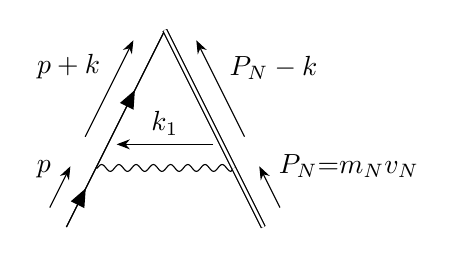
\begin{tikzpicture}[baseline=($(p1)!0.5!(x)$)]
		\begin{feynman}
			\vertex (p1);
			\vertex[right=2.5cm of p1] (p2);
			\vertex at ($(p1)!0.5!(p2)+(0,2.5cm)$) (x) ;
			\vertex at ($(p1)!0.3!(x)$) (y1);
			\vertex at ($(p2)!0.3!(x)$) (z1);
			%
			\diagram* {
			(p1) -- [] (x);
			(p2) -- [double distance=1pt] (x);
			(y1) -- [photon,rmomentum=$k_1$] (z1);
			(p1) -- [momentum=\(p\),fermion] (y1);
			(p2) -- [momentum'=$P_{N}\text{=}m_{N}v_{N}$,double distance=1pt] (z1);
			(y1) -- [momentum=\(p+k\),fermion] (x);
			(z1) -- [momentum'=\(P_{N}-k\),double distance=1pt] (x);
			};
		\end{feynman}
	\end{tikzpicture}
\end{align*}
which doesn't have logarithm divergence. We can rigorously prove that so long as there's no dynamic photon, NRQED has no logarithmic divergence at one loop order (at least for this problem we're considering).
\subsection{NNLO}
\begin{align*}
	- & 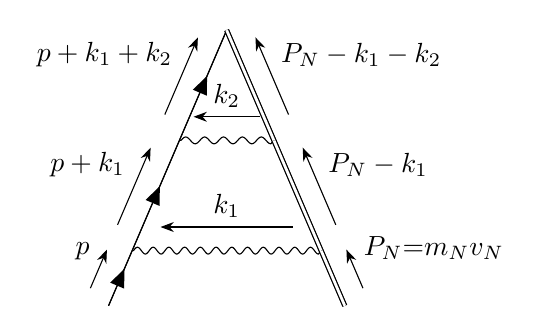
\begin{tikzpicture}[baseline=($(p1)!0.5!(x)$)]
		\begin{feynman}
			\vertex (p1);
			\vertex[right=3cm of p1] (p2);
			\vertex at ($(p1)!0.5!(p2)+(0,3.5cm)$) (x) ;
			\vertex at ($(p1)!0.2!(x)$) (y1);
			\vertex at ($(p2)!0.2!(x)$) (z1);
			\vertex at ($(p1)!0.6!(x)$) (y2);
			\vertex at ($(p2)!0.6!(x)$) (z2);
			%
			\diagram* {
			(p1) -- [] (x);
			(p2) -- [double distance=1pt] (x);
			(y1) -- [photon,rmomentum=$k_1$] (z1);
			(y2) -- [photon,rmomentum=$k_2$] (z2);
			(p1) -- [momentum=\(p\),fermion] (y1);
			(p2) -- [momentum'=$P_{N}\text{=}m_{N}v_{N}$,double distance=1pt] (z1);
			(y1) -- [momentum=\(p+k_1\),fermion] (y2);
			(z1) -- [momentum'=\(P_{N}-k_1\),double distance=1pt] (z2);
			(y2) -- [momentum=\(p+k_1+k_2\),fermion] (x);
			(z2) -- [momentum'=\(P_{N}-k_1-k_2\),double distance=1pt] (x);
			};
		\end{feynman}
	\end{tikzpicture}=0+\text{finite terms}                                                  \\
	  & 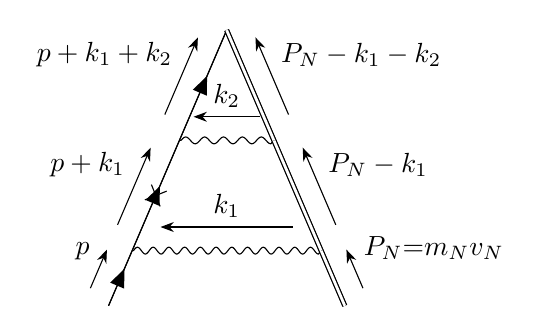
\begin{tikzpicture}[baseline=($(p1)!0.5!(x)$)]
		\begin{feynman}
			\vertex (p1);
			\vertex[right=3cm of p1] (p2);
			\vertex at ($(p1)!0.5!(p2)+(0,3.5cm)$) (x) ;
			\vertex at ($(p1)!0.2!(x)$) (y1);
			\vertex at ($(p2)!0.2!(x)$) (z1);
			\vertex at ($(p1)!0.6!(x)$) (y2);
			\vertex at ($(p2)!0.6!(x)$) (z2);
			\vertex at ($(y1)!0.5!(z1)$) (t);
			%
			\diagram* {
			(p1) -- [] (x);
			(p2) -- [double distance=1pt] (x);
			(y1) -- [photon,rmomentum=$k_1$] (z1);
			(y2) -- [photon,rmomentum=$k_2$] (z2);
			(p1) -- [momentum=\(p\),fermion] (y1);
			(p2) -- [momentum'=$P_{N}\text{=}m_{N}v_{N}$,double distance=1pt] (z1);
			(y1) -- [momentum=\(p+k_1\),insertion=0.5,fermion] (y2);
			(z1) -- [momentum'=\(P_{N}-k_1\),double distance=1pt] (z2);
			(y2) -- [momentum=\(p+k_1+k_2\),fermion] (x);
			(z2) -- [momentum'=\(P_{N}-k_1-k_2\),double distance=1pt] (x);
			};
		\end{feynman}
	\end{tikzpicture}
	%=4m^2\mu^{2\epsilon}Z^2e^4\int\frac{\dd^3\vb{k_1}}{(2\pi)^3}\frac{\dd^3\vb{k_2}}{(2\pi)^3}\frac{1}{\vb{\abs{k_1-p}}^2}\frac{1}{\vb{\abs{k_2-k_1}}^2}\frac{\vb{\abs{k_1}}^4/4m^2}{[\vb{\abs{k_1}}^2-2mE]^2}\frac{1}{\vb{\abs{k_2}}^2-2mE}\\
	=Z^2\a^2(\frac{1}{2(3-d)}+\log \mu)+\text{finite terms}\\
	  & 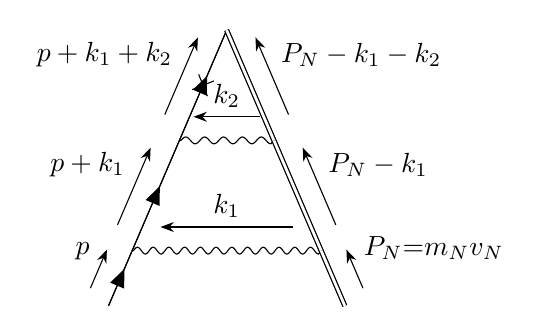
\begin{tikzpicture}[baseline=($(p1)!0.5!(x)$)]
		\begin{feynman}
			\vertex (p1);
			\vertex[right=3cm of p1] (p2);
			\vertex at ($(p1)!0.5!(p2)+(0,3.5cm)$) (x) ;
			\vertex at ($(p1)!0.2!(x)$) (y1);
			\vertex at ($(p2)!0.2!(x)$) (z1);
			\vertex at ($(p1)!0.6!(x)$) (y2);
			\vertex at ($(p2)!0.6!(x)$) (z2);
			\vertex at ($(y1)!0.5!(z1)$) (t);
			%
			\diagram* {
			(p1) -- [] (x);
			(p2) -- [double distance=1pt] (x);
			(y1) -- [photon,rmomentum=$k_1$] (z1);
			(y2) -- [photon,rmomentum=$k_2$] (z2);
			(p1) -- [momentum=\(p\),fermion] (y1);
			(p2) -- [momentum'=$P_{N}\text{=}m_{N}v_{N}$,double distance=1pt] (z1);
			(y1) -- [momentum=\(p+k_1\),fermion] (y2);
			(z1) -- [momentum'=\(P_{N}-k_1\),double distance=1pt] (z2);
			(y2) -- [momentum=\(p+k_1+k_2\),insertion=0.5,fermion] (x);
			(z2) -- [momentum'=\(P_{N}-k_1-k_2\),double distance=1pt] (x);
			};
		\end{feynman}
	\end{tikzpicture}
	% =4m^2   \mu^{2\epsilon}Z^2e^4\int\frac{\dd^3\vb{k_1}}{(2\pi)^3}\frac{\dd^3\vb{k_2}}{(2\pi)^3}\frac{1}{\vb{\abs{k_1-p}}^2}\frac{1}{\vb{\abs{k_2-k_1}}^2}\frac{1}{\vb{\abs{k_1}}^2-2mE}\frac{\vb{\abs{k_2}}^4/4m^2}{[\vb{\abs{k_2}}^2-2mE]^2}\\
	=0+\text{finite terms}\\
	  & 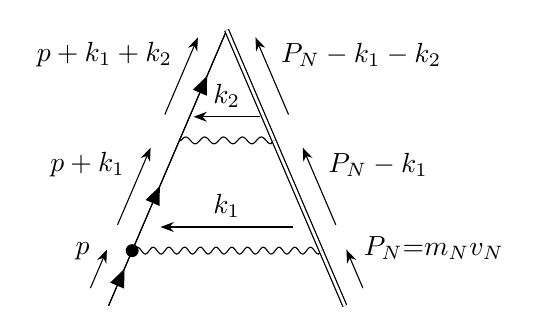
\begin{tikzpicture}[baseline=($(p1)!0.5!(x)$)]
		\begin{feynman}
			\vertex (p1);
			\vertex[right=3cm of p1] (p2);
			\vertex at ($(p1)!0.5!(p2)+(0,3.5cm)$) (x) ;
			\vertex at ($(p1)!0.2!(x)$) (y1);
			\node [dot] at ($(y1)$) (tmp);
			\vertex at ($(p2)!0.2!(x)$) (z1);
			\vertex at ($(p1)!0.6!(x)$) (y2);
			\vertex at ($(p2)!0.6!(x)$) (z2);
			%
			\diagram* {
			(p1) -- [] (x);
			(p2) -- [double distance=1pt] (x);
			(y1) -- [photon,rmomentum=$k_1$] (z1);
			(y2) -- [photon,rmomentum=$k_2$] (z2);
			(p1) -- [momentum=\(p\),fermion] (y1);
			(p2) -- [momentum'=$P_{N}\text{=}m_{N}v_{N}$,double distance=1pt] (z1);
			(y1) -- [momentum=\(p+k_1\),fermion] (y2);
			(z1) -- [momentum'=\(P_{N}-k_1\),double distance=1pt] (z2);
			(y2) -- [momentum=\(p+k_1+k_2\),fermion] (x);
			(z2) -- [momentum'=\(P_{N}-k_1-k_2\),double distance=1pt] (x);
			};
		\end{feynman}
	\end{tikzpicture}= Z^2\alpha ^2(\frac{1}{4 (d-3)}-\frac{\log\mu}{2})+\text{finite terms} \\
	  & 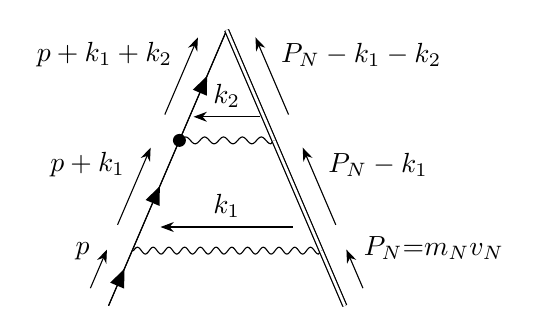
\begin{tikzpicture}[baseline=($(p1)!0.5!(x)$)]
		\begin{feynman}
			\vertex (p1);
			\vertex[right=3cm of p1] (p2);
			\vertex at ($(p1)!0.5!(p2)+(0,3.5cm)$) (x) ;
			\vertex at ($(p1)!0.2!(x)$) (y1);
			\vertex at ($(p2)!0.2!(x)$) (z1);
			\vertex at ($(p1)!0.6!(x)$) (y2);
			\node [dot] at ($(y2)$) (tmp);
			\vertex at ($(p2)!0.6!(x)$) (z2);
			%
			\diagram* {
			(p1) -- [] (x);
			(p2) -- [double distance=1pt] (x);
			(y1) -- [photon,rmomentum=$k_1$] (z1);
			(y2) -- [photon,rmomentum=$k_2$] (z2);
			(p1) -- [momentum=\(p\),fermion] (y1);
			(p2) -- [momentum'=$P_{N}\text{=}m_{N}v_{N}$,double distance=1pt] (z1);
			(y1) -- [momentum=\(p+k_1\),fermion] (y2);
			(z1) -- [momentum'=\(P_{N}-k_1\),double distance=1pt] (z2);
			(y2) -- [momentum=\(p+k_1+k_2\),fermion] (x);
			(z2) -- [momentum'=\(P_{N}-k_1-k_2\),double distance=1pt] (x);
			};
		\end{feynman}
	\end{tikzpicture}= Z^2\alpha ^2(\frac{1}{2 (d-3)}-\log\mu)\text{finite terms}
\end{align*}
After summing those all together, we can see that the coefficient of $\log\mu$ is exact the same as which of $\log\Lambda$ in the Schr\"odinger wavefunction with $\vbp^4$ relativistic correction and of $\log r$ in Klein-Gordon wavefunction. 
\section{OPE}
The relativistic correction part is the same as scalar ones. 
\begin{align*}
	&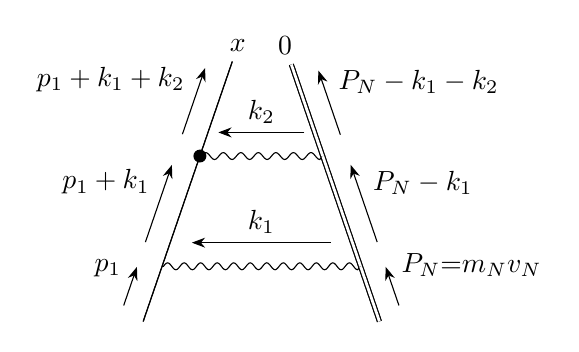
\begin{tikzpicture}[baseline=($(p1)!0.5!(x)$)]
		\begin{feynman}
		\vertex (p1);
		\vertex[right=3cm of p1] (p2);
		\vertex at ($(p1)!0.4!(p2)+(0,3.5cm)$) (x) {$x$};
		\vertex at ($(p1)!0.6!(p2)+(0,3.5cm)$) (0) {$0$};
		\vertex at ($(p1)!0.2!(x)$) (y1);
		\vertex at ($(p2)!0.2!(0)$) (z1);
		\vertex at ($(p1)!0.6!(x)$) (y2);
		\vertex at ($(p2)!0.6!(0)$) (z2);
		\node [dot] at ($(y2)$) (tmp);
		%
		\diagram* {
		  (p1) -- [] (x);
		  (p2) -- [double distance=1pt] (0);
		  (y1) -- [photon,rmomentum=$k_1$] (z1);
		  (y2) -- [photon,rmomentum=$k_2$] (z2);
		  (p1) -- [momentum=\(p_{1}\)] (y1);
		  (p2) -- [momentum'=$P_{N}\text{=}m_{N}v_{N}$,double distance=1pt] (z1);
		  (y1) -- [momentum=\(p_{1}+k_1\)] (y2);
		  (z1) -- [momentum'=\(P_{N}-k_1\),double distance=1pt] (z2);
		  (y2) -- [momentum=\(p_{1}+k_1+k_2\)] (x);
		  (z2) -- [momentum'=\(P_{N}-k_1-k_2\),double distance=1pt] (0);
		};
		\end{feynman}
	  \end{tikzpicture}-
	  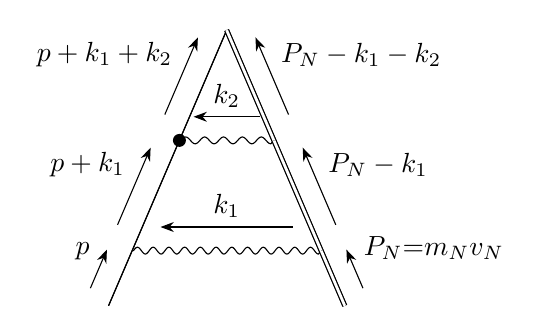
\begin{tikzpicture}[baseline=($(p1)!0.5!(x)$)]
		\begin{feynman}
			\vertex (p1);
			\vertex[right=3cm of p1] (p2);
			\vertex at ($(p1)!0.5!(p2)+(0,3.5cm)$) (x) ;
			\vertex at ($(p1)!0.2!(x)$) (y1);
			\vertex at ($(p2)!0.2!(x)$) (z1);
			\vertex at ($(p1)!0.6!(x)$) (y2);
			\vertex at ($(p2)!0.6!(x)$) (z2);
			\vertex at ($(y1)!0.5!(z1)$) (t);
			\node [dot] at ($(y2)$) (tmp);
			%
			\diagram* {
			(p1) -- [] (x);
			(p2) -- [double distance=1pt] (x);
			(y1) -- [photon,rmomentum=$k_1$] (z1);
			(y2) -- [photon,rmomentum=$k_2$] (z2);
			(p1) -- [momentum=\(p\)] (y1);
			(p2) -- [momentum'=$P_{N}\text{=}m_{N}v_{N}$,double distance=1pt] (z1);
			(y1) -- [momentum=\(p+k_1\)] (y2);
			(z1) -- [momentum'=\(P_{N}-k_1\),double distance=1pt] (z2);
			(y2) -- [momentum=\(p+k_1+k_2\)] (x);
			(z2) -- [momentum'=\(P_{N}-k_1-k_2\),double distance=1pt] (x);
			};
		\end{feynman}
	\end{tikzpicture}\\
	=&-4m^2\mu^{2\epsilon}Z^2e^4
	\int\frac{\dd^3\vb{k_1}}{(2\pi)^3}\frac{\dd^3\vb{k_2}}{(2\pi)^3}\bqty{e^{-i\vb{k}_2\cdot\vb{x}}-1}\frac{1}{\vb{\abs{k_1-p}}^2}\frac{1}{\vb{\abs{k_2-k_1}}^2}\frac{1}{\vb{\abs{k_1}}^2-2mE}\frac{(\vb{k}_1+\vb{k}_2)^2/8m^2}{\vb{\abs{k_2}}^2-2mE}
\end{align*}
\begin{align*}
	&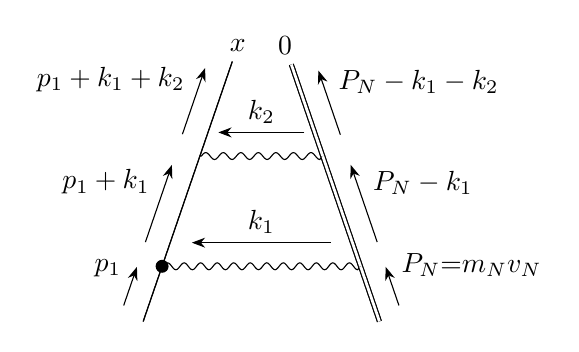
\begin{tikzpicture}[baseline=($(p1)!0.5!(x)$)]
		\begin{feynman}
		\vertex (p1);
		\vertex[right=3cm of p1] (p2);
		\vertex at ($(p1)!0.4!(p2)+(0,3.5cm)$) (x) {$x$};
		\vertex at ($(p1)!0.6!(p2)+(0,3.5cm)$) (0) {$0$};
		\vertex at ($(p1)!0.2!(x)$) (y1);
		\vertex at ($(p2)!0.2!(0)$) (z1);
		\vertex at ($(p1)!0.6!(x)$) (y2);
		\vertex at ($(p2)!0.6!(0)$) (z2);
		\node [dot] at ($(y1)$) (tmp);
		%
		\diagram* {
		  (p1) -- [] (x);
		  (p2) -- [double distance=1pt] (0);
		  (y1) -- [photon,rmomentum=$k_1$] (z1);
		  (y2) -- [photon,rmomentum=$k_2$] (z2);
		  (p1) -- [momentum=\(p_{1}\)] (y1);
		  (p2) -- [momentum'=$P_{N}\text{=}m_{N}v_{N}$,double distance=1pt] (z1);
		  (y1) -- [momentum=\(p_{1}+k_1\)] (y2);
		  (z1) -- [momentum'=\(P_{N}-k_1\),double distance=1pt] (z2);
		  (y2) -- [momentum=\(p_{1}+k_1+k_2\)] (x);
		  (z2) -- [momentum'=\(P_{N}-k_1-k_2\),double distance=1pt] (0);
		};
		\end{feynman}
	  \end{tikzpicture}-
	  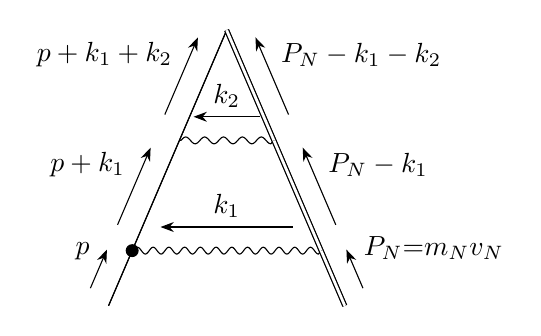
\begin{tikzpicture}[baseline=($(p1)!0.5!(x)$)]
		\begin{feynman}
			\vertex (p1);
			\vertex[right=3cm of p1] (p2);
			\vertex at ($(p1)!0.5!(p2)+(0,3.5cm)$) (x) ;
			\vertex at ($(p1)!0.2!(x)$) (y1);
			\vertex at ($(p2)!0.2!(x)$) (z1);
			\vertex at ($(p1)!0.6!(x)$) (y2);
			\vertex at ($(p2)!0.6!(x)$) (z2);
			\vertex at ($(y1)!0.5!(z1)$) (t);
			\node [dot] at ($(y1)$) (tmp);
			%
			\diagram* {
			(p1) -- [] (x);
			(p2) -- [double distance=1pt] (x);
			(y1) -- [photon,rmomentum=$k_1$] (z1);
			(y2) -- [photon,rmomentum=$k_2$] (z2);
			(p1) -- [momentum=\(p\)] (y1);
			(p2) -- [momentum'=$P_{N}\text{=}m_{N}v_{N}$,double distance=1pt] (z1);
			(y1) -- [momentum=\(p+k_1\)] (y2);
			(z1) -- [momentum'=\(P_{N}-k_1\),double distance=1pt] (z2);
			(y2) -- [momentum=\(p+k_1+k_2\)] (x);
			(z2) -- [momentum'=\(P_{N}-k_1-k_2\),double distance=1pt] (x);
			};
		\end{feynman}
	\end{tikzpicture}\\
	=&-4m^2\mu^{2\epsilon}Z^2e^4
	\int\frac{\dd^3\vb{k_1}}{(2\pi)^3}\frac{\dd^3\vb{k_2}}{(2\pi)^3}\bqty{e^{-i\vb{k}_2\cdot\vb{x}}-1}\frac{1}{\vb{\abs{k_1-p}}^2}\frac{1}{\vb{\abs{k_2-k_1}}^2}\frac{(\vb{p}+\vb{k}_1)^2/8m^2}{\vb{\abs{k_1}}^2-2mE}\frac{1}{\vb{\abs{k_2}}^2-2mE}
\end{align*}

\end{document}
